% Options for packages loaded elsewhere
\PassOptionsToPackage{unicode}{hyperref}
\PassOptionsToPackage{hyphens}{url}
%
\documentclass[
  ignorenonframetext,
  aspectratio=169]{beamer}
\usepackage{pgfpages}
\setbeamertemplate{caption}[numbered]
\setbeamertemplate{caption label separator}{: }
\setbeamercolor{caption name}{fg=normal text.fg}
\beamertemplatenavigationsymbolsempty
% Prevent slide breaks in the middle of a paragraph
\widowpenalties 1 10000
\raggedbottom
\setbeamertemplate{part page}{
  \centering
  \begin{beamercolorbox}[sep=16pt,center]{part title}
    \usebeamerfont{part title}\insertpart\par
  \end{beamercolorbox}
}
\setbeamertemplate{section page}{
  \centering
  \begin{beamercolorbox}[sep=12pt,center]{part title}
    \usebeamerfont{section title}\insertsection\par
  \end{beamercolorbox}
}
\setbeamertemplate{subsection page}{
  \centering
  \begin{beamercolorbox}[sep=8pt,center]{part title}
    \usebeamerfont{subsection title}\insertsubsection\par
  \end{beamercolorbox}
}
\AtBeginPart{
  \frame{\partpage}
}
\AtBeginSection{
  \ifbibliography
  \else
    \frame{\sectionpage}
  \fi
}
\AtBeginSubsection{
  \frame{\subsectionpage}
}
\usepackage{lmodern}
\usepackage{amssymb,amsmath}
\usepackage{ifxetex,ifluatex}
\ifnum 0\ifxetex 1\fi\ifluatex 1\fi=0 % if pdftex
  \usepackage[T1]{fontenc}
  \usepackage[utf8]{inputenc}
  \usepackage{textcomp} % provide euro and other symbols
\else % if luatex or xetex
  \usepackage{unicode-math}
  \defaultfontfeatures{Scale=MatchLowercase}
  \defaultfontfeatures[\rmfamily]{Ligatures=TeX,Scale=1}
\fi
\usetheme[]{Frankfurt}
\usecolortheme{beaver}
% Use upquote if available, for straight quotes in verbatim environments
\IfFileExists{upquote.sty}{\usepackage{upquote}}{}
\IfFileExists{microtype.sty}{% use microtype if available
  \usepackage[]{microtype}
  \UseMicrotypeSet[protrusion]{basicmath} % disable protrusion for tt fonts
}{}
\makeatletter
\@ifundefined{KOMAClassName}{% if non-KOMA class
  \IfFileExists{parskip.sty}{%
    \usepackage{parskip}
  }{% else
    \setlength{\parindent}{0pt}
    \setlength{\parskip}{6pt plus 2pt minus 1pt}}
}{% if KOMA class
  \KOMAoptions{parskip=half}}
\makeatother
\usepackage{xcolor}
\IfFileExists{xurl.sty}{\usepackage{xurl}}{} % add URL line breaks if available
\IfFileExists{bookmark.sty}{\usepackage{bookmark}}{\usepackage{hyperref}}
\hypersetup{
  pdftitle={Climate change and its impacts on mountain agriculture},
  pdfauthor={Deependra Dhakal},
  hidelinks,
  pdfcreator={LaTeX via pandoc}}
\urlstyle{same} % disable monospaced font for URLs
\newif\ifbibliography
\setlength{\emergencystretch}{3em} % prevent overfull lines
\providecommand{\tightlist}{%
  \setlength{\itemsep}{0pt}\setlength{\parskip}{0pt}}
\setcounter{secnumdepth}{-\maxdimen} % remove section numbering
\usepackage{booktabs}
\usepackage{longtable}
\usepackage{array}
\usepackage{multirow}
\usepackage{wrapfig}
\usepackage{float}
\usepackage{colortbl}
\usepackage{pdflscape}
\usepackage{tabu}
\usepackage{threeparttable}
\usepackage{threeparttablex}
\usepackage[normalem]{ulem}
\usepackage{makecell}
\usepackage{xcolor}
\usepackage{tikz} % required for image opacity change
\usepackage[absolute,overlay]{textpos} % for text formatting

% this font option is amenable for beamer
\setbeamerfont{caption}{size=\tiny}

\title{Climate change and its impacts on mountain agriculture}
\author{Deependra Dhakal}
\date{Academic year 2019-2020}
\institute{GAASC, Baitadi \and Tribhuwan University}

\begin{document}
\frame{\titlepage}

\begin{frame}[allowframebreaks]
  \tableofcontents[hideallsubsections]
\end{frame}
\hypertarget{general-impacts}{%
\section{General impacts}\label{general-impacts}}

\begin{frame}{}
\protect\hypertarget{section}{}
\begin{center}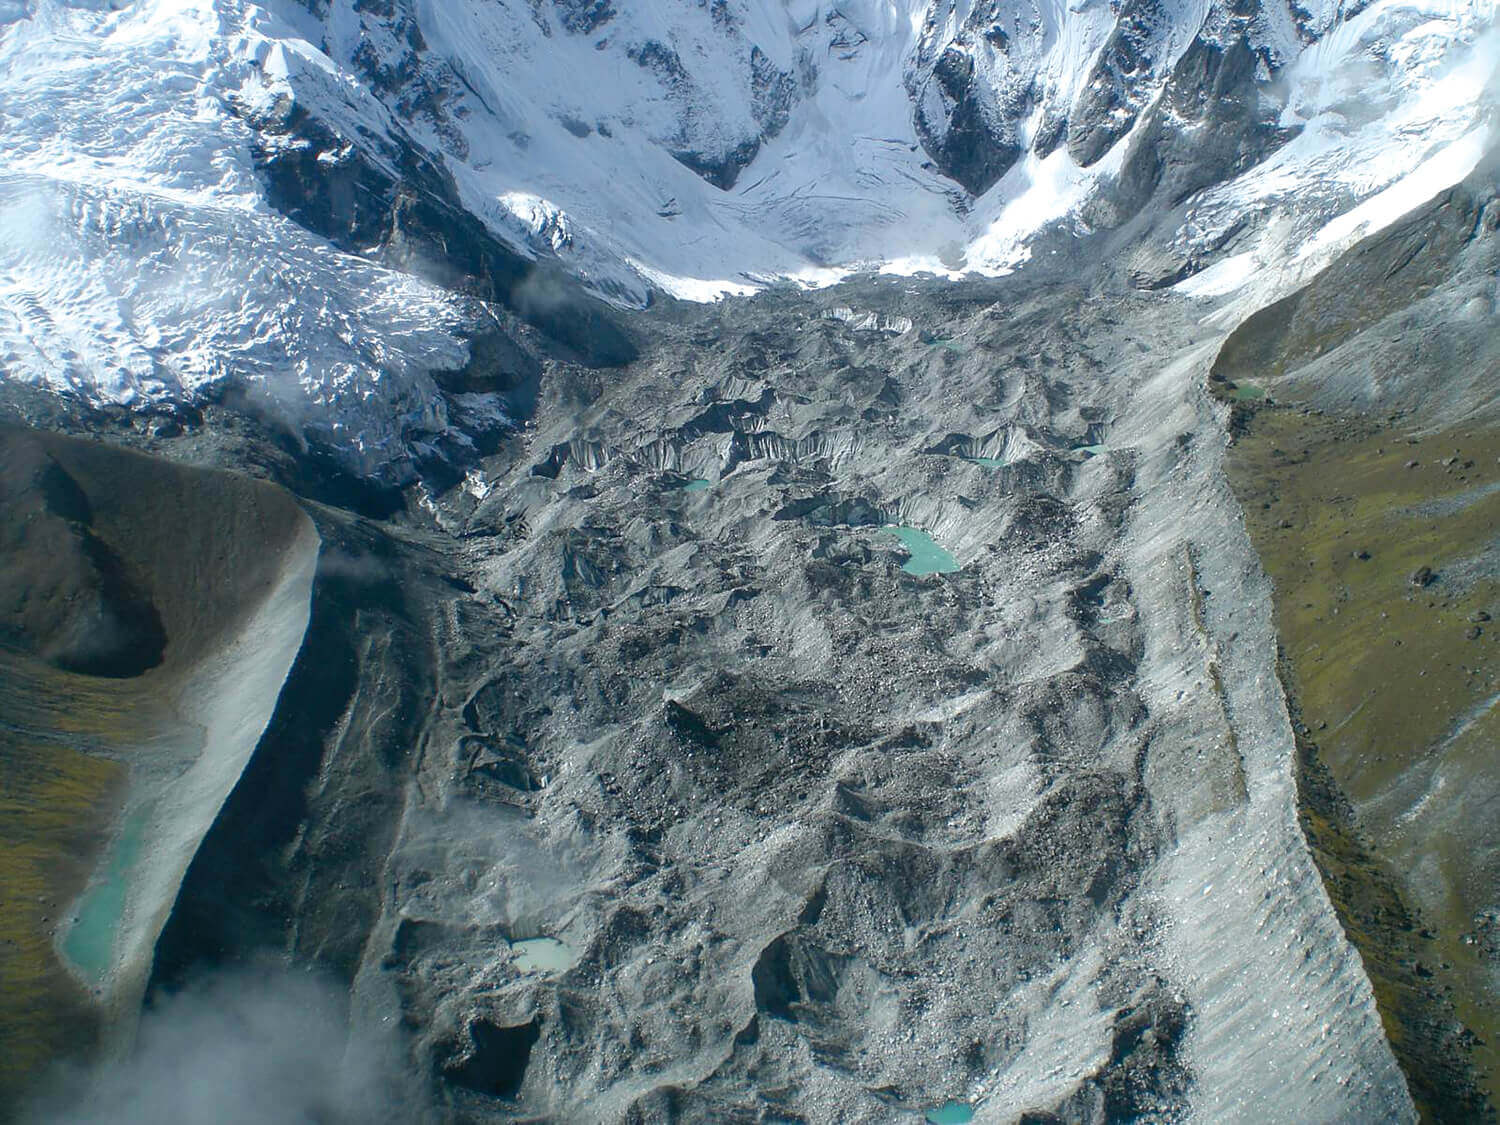
\includegraphics[width=0.7\linewidth]{../images/mountain_agriculture/Climate-change-impact-on-the-Himalaya} \end{center}
\end{frame}

\begin{frame}{For higher latitudes}
\protect\hypertarget{for-higher-latitudes}{}
\begin{itemize}
\tightlist
\item
  Some species of vegetation require not only a stable climate but a
  narrow range of meteorological extremes such as high and low
  temperatures, precipitation, and soil moisture.
\item
  The Intergovernmental Panel on Climate Change, created by the United
  Nations in 1988, has concluded that over the next 50 years projected
  changes in regional temperatures and precipitation could cause
  climatic zones to shift hundreds of kilometers toward the polar
  regions.
\item
  Some biotic communities may be capable of adapting to a climatic shift
  of such magnitude, while others would experience substantial loss that
  could include some species extinction.
\item
  In higher altitutes, impacts for forest line.
\item
  the permafrost that presently underlies the 20--25\% of the Northern
  Hemisphere that is perenially frigid may begin to thaw during the next
  40--50 years. Degradation of the permafrost cover would damage
  high-latitude surface ecosystems, destabilize terrain, and cause soil
  erosion.
\end{itemize}
\end{frame}

\begin{frame}{}
\protect\hypertarget{section-1}{}
\begin{figure}
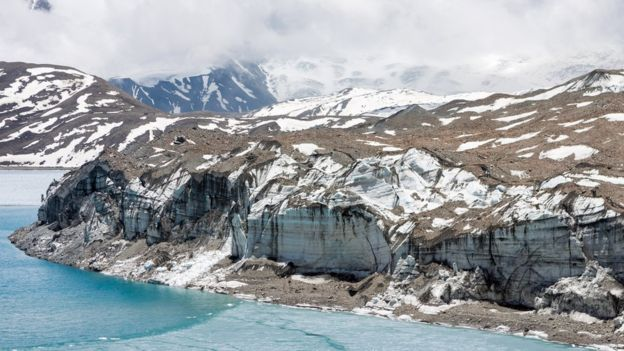
\includegraphics[width=0.7\linewidth]{../images/mountain_agriculture/himalayan_glacier_melting} \caption{Melting of Himalayan glacial cover}\label{fig:climate-change-everest}
\end{figure}
\end{frame}

\begin{frame}{To crops}
\protect\hypertarget{to-crops}{}
\begin{itemize}
\tightlist
\item
  Major effects due to increasing concentration of \(CO_2\). The level
  of atmospheric \(CO_2\) in Europe has increased from about
  \(280 \mu mol~\mathrm{CO_2}~mol^{-1}\) before the industrial era to
  \(358 \mu mol\) \(\mathrm{CO_2}~mol^{-1}\) in 1995 .
\item
  This trend is expected to continue and result in an increase to over
  \(700~\mu~mol~mol^{-1}\) by the end of the next century if no steps
  are taken to limit emissions.
\item
  In parallel with the recent trend of rising atmospheric
  {[}\(CO_2\){]}, ozone (\(O_3\)) also has increased and is regarded as
  being one of the most phytotoxic of the air pollutants commonly
  encountered in the developed countries of the Northern Hemisphere.
\end{itemize}
\end{frame}

\begin{frame}{}
\protect\hypertarget{section-2}{}
\begin{itemize}
\tightlist
\item
  Plants respond to elevated \(CO_2\) levels by:

  \begin{itemize}
  \tightlist
  \item
    Changes in growth and yield
  \item
    Structure and anatomy
  \item
    Photosynthetic and respiratory gas exchange
  \item
    C and N assimilation
  \item
    Transpirational and water use efficiency and hence turgor pressure
  \end{itemize}
\item
  Phytotron experiments, Free air \(CO_2\) enrichment (FACE) technique.
\item
  Among the wide range of \(C_3\) species that have been examined,
  including virtually all crop and forest species of northern latitudes,
  the photosynthesis of some 95\% is not saturated by the present
  {[}\(CO_2\){]}. \(C_3\) plants require 800--1000
  \(\mu~mol~mol^{-1}~CO_2\) for saturation of photosynthesis. Almost all
  show significant increases in photosynthesis and dry matter production
  in response to an increase in {[}\(CO_2\){]} of between 500 and 1000
  \(\mu~mol~mol^{-1}~CO_2\). A doubling of {[}\(CO_2\){]} from 330 to
  660 \(\mu~mol~mol^{-1}~CO_2\) increases the productivity of crops and
  \(C_3\) plants by 33--41\% .
\end{itemize}
\end{frame}

\begin{frame}{}
\protect\hypertarget{section-3}{}
\begin{itemize}
\tightlist
\item
  Although the net photosynthesis assimilation increases by an average
  of 50\% in the short term, the plant weight increases by only 40\%
  over a long period. Such stimulation is modest compared with what
  might be expected on the basis of short-term increases in carbon
  fixation at high {[}\(CO_2\){]}. Also, there is much evidence that the
  initial \(CO_2\) stimulation of photosynthesis is not maintained and
  that downregulation of photosynthesis caused by acclimation occurs
  after prolonged exposure to high \(CO_2\) concentration.
\item
  Increases above ground biomass in wheat, faba bean, however no
  significant change in HI.
\end{itemize}
\end{frame}

\hypertarget{specific-impacts}{%
\section{Specific impacts}\label{specific-impacts}}

\begin{frame}{In rice}
\protect\hypertarget{in-rice}{}
\begin{itemize}
\tightlist
\item
  The sensitivity of rice reproductive growth stages in terms of yield
  reduction or sensitivity to drought was ranked in the following order:
  (a) flowering, (b) gametogenesis, (c) panicle initiation, and (d)
  grain fill.
\item
  Drought stress reduces biomass accumulation both at ambient and
  elevated \(CO_2\) levels.
\item
  Carbon dioxide enrichment significantly increased both the canopy net
  photosynthetic rate and water-use efficiency, whereas reducing
  evapotranspiration by about 10\%. This water saving under
  {[}\(CO_2\){]} enrichment allowed photosynthesis to continue for about
  1--2 days longer during drought in the enriched compared with the
  ambient {[}\(CO_2\){]} control treatment.
\item
  These results indicate that, in the absence of other potential climate
  change factors, such as increased air temperature, rice grown in the
  next century may use less water, use water more efficiently, and
  become better able to avoid drought in some situations.
\end{itemize}
\end{frame}

\begin{frame}{Climate change threats to glacial region of Hindu Kush
Himalayas}
\protect\hypertarget{climate-change-threats-to-glacial-region-of-hindu-kush-himalayas}{}
\begin{itemize}
\tightlist
\item
  Even if the world limits the temperature rise to 1.5\(^\circ C\) this
  century, at least one third of the ice would go\footnote<.->{Climate
    change poses a growing threat to the glaciers found in the Hindu
    Kush and Himalayan mountain ranges}.
\item
  The glaciers are a critical water source for 250 million people living
  across eight different countries.
\item
  Impacts on people in the region, already one of the world's most
  fragile and hazard-prone mountain regions, will range from worsened
  air pollution to an increase in extreme weather events.
\item
  The HK region covers some 3,500km across Afghanistan, Bangladesh,
  Bhutan, China, India, Myanmar, Nepal and Pakistan.
\item
  Glaciers feed world's most important river systems.
\item
  Impact for the 1.65 billion people living in the river valleys below,
  with rising vulnerability to flooding and destruction of crops.
\end{itemize}
\end{frame}

\begin{frame}{}
\protect\hypertarget{section-4}{}
\begin{itemize}
\tightlist
\item
  Himalayan peaks are warming between 0.3 to 0.7\(^\circ C\) faster than
  the global average,
\item
  Measurements show that glaciers in the Central and Eastern Himalaya
  are shrinking at 40cm/year, and some are receding up to
  30m/year\footnote<.->{\href{https://www.nepalitimes.com/banner/a-terrifying-assessment-of-himalayan-melting/}{Terrifying
    assessment of himalayan melting}}.
\item
  The hydro-meteorological impact of climate change will go beyond
  countries like Nepal or Bhutan.
\end{itemize}
\end{frame}

\begin{frame}{Nepal's fragility}
\protect\hypertarget{nepals-fragility}{}
\begin{itemize}
\tightlist
\item
  Largely fed by South Asian Monsoon system, but the mountainscape and
  the orographic rainfall pattern are intimately related.
\item
  Dramatic variation in altitudinal differences over a short distance
  complicates the precipitation dynamics.
\item
  Meteorological information system and hydrological set ups are poor
  and very limited in their information value.
\item
  The diversity in Nepal's climate is matched by the diversity of its
  multiple ecosystems and flora and fauna species.
\item
  Each of these many socio-economic systems is custom-tailored to take
  advantage of the opportunities offered by specific micro-climates and
  localised ecosystems and to respond to the constraints they impose on
  livelihoods.
\end{itemize}
\end{frame}

\begin{frame}{}
\protect\hypertarget{section-5}{}
\begin{itemize}
\tightlist
\item
  The livelihoods of over three-quarters of all Nepalis are based on
  agriculture and forest resources, and almost 65 percent of agriculture
  is rain-fed (MoPE, 2000).\\
\item
  Yet only 21 \% of Nepal's area is cultivable and the irrigable
  agriculture depends on the types of local surface sources, most likely
  to be affected by erratic rainfall.
\item
  Country hosts more than 6,000 rivers and rivulets, with a total of
  45,000 km in length, support irrigated agriculture and other
  livelihoods. Rivers wreak havoc in valleys and in the tarai when they
  overflow.
\item
  There are 2323 glacial lakes covering 75 sq. km area.
\item
  Rice based food system provides for much of the staple in Hills and
  Terai\footnote<.->{\url{https://kathmandupost.com/money/2018/08/31/bumper-paddy-crop-expected-this-year}}.
\item
  As regions become drier, Nepalese forest cover of 40\% is at increased
  risk of fire. Already, in the spring of 2009, smoke from fires
  blanketed much of the Himalaya, from Kashmir in the west to Meghalaya
  in the east.
\end{itemize}
\end{frame}

\begin{frame}{}
\protect\hypertarget{section-6}{}
\begin{itemize}
\tightlist
\item
  Himalayas and hills have young soils, due to flashy runoff and debris
  flow after precipitation, fertility of upper region decends
  immediately.
\item
  In mostly the flooded plains and downstream sites of landslides,
  sediment transfer will render land uncultivable.
\item
  Shifting river channels often inundate arable fields and occassionally
  breach the embankments to completely sweep away the fertile basins.
\item
  Long term impacts on himalayan livelihood that depends on NTFPs; loss
  of forest, poorer water supplies. Lesser groundwater recharge owing to
  lesser forest coverage.
\item
  With lack of forest supplies and ebb in vegetation or wildlife
  divesity in forests or largely natural spaces, wildlife will face
  habitat disruption and might more freqently meet with human
  trespassing.
\end{itemize}
\end{frame}

\begin{frame}{}
\protect\hypertarget{section-7}{}
\begin{figure}
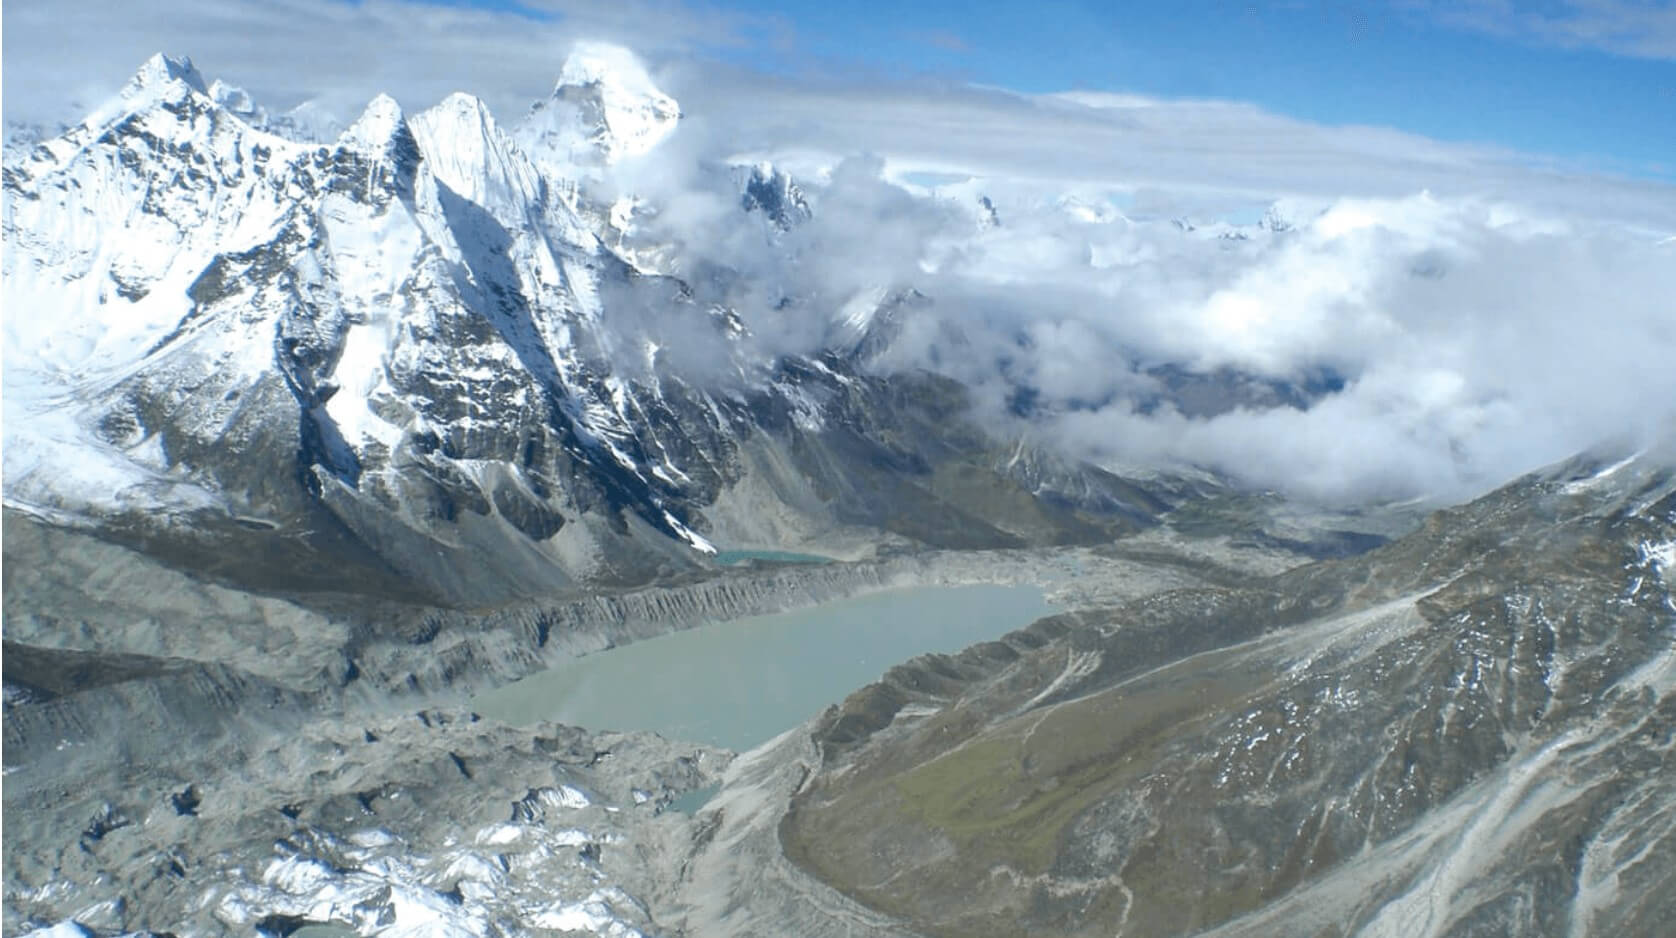
\includegraphics[width=0.65\linewidth]{../images/mountain_agriculture/receding_imja_lake_everest_region} \caption{Receding imja lake at Mount Everest region}\label{fig:imja-lake-receding}
\end{figure}
\end{frame}

\hypertarget{assessment-and-projections}{%
\section{Assessment and projections}\label{assessment-and-projections}}

\begin{frame}{}
\protect\hypertarget{section-8}{}
\begin{itemize}
\tightlist
\item
  Mirza and Dixit (1997) found that climate change in the Ganga and
  Brahmaputra basins is likely to change river flows, which in turn will
  affect low flows, drought, flood and sedimentation processes.
\item
  In 1999 Shrestha et al.~suggested that temperatures are increasing in
  Nepal and that rainfall is becoming more variable.
\item
  In 2009, a modeling exercise conducted by team of Nepali, American,
  British, Pakistani and Bangladeshi experts (NCVST,2009) using the
  emissions scenarios in the IPCC's special report (2007) found that the
  temperature will indeed increase in the mid-hills and that this region
  is likely to grow more arid in the non-monsoon seasons.
\end{itemize}
\end{frame}

\begin{frame}{}
\protect\hypertarget{section-9}{}
\begin{itemize}
\tightlist
\item
  During 2008-2008 winter drought, most monitoring stations received
  less than 50\% of normal rainfall, 30\% recorded no precipitation at
  all and temperatures were 1-2\(^\circ C\) above average. At the
  national level, wheat and barley production decreased by 14.5\% and
  17.3\% respectively and the 2009 maize production was also seriously
  affected.
\item
  Global circulation model (GCM) projections indicate:

  \begin{itemize}
  \tightlist
  \item
    that the temperature over Nepal will increase between
    0.5\(^\circ C\) and 2.0\(^\circ C\) with a multi-model mean of
    1.4\(^\circ C\), by the 2030s and between 3.0\(^\circ C\) and
    6.3\(^\circ C\), with a multi-model mean of 4.7\(^\circ C\), by the
    2090s. GCM outputs suggest that extremely hot days (the hottest 5\%
    of days in the period from 1970 to 1999) are projected to increase
    by up to 55\% by the 2060s and up to 70\% by the 2090s.
  \item
    that extremely hot nights (the hottest 5\% of nights in the period
    from 1970 to 1999) are projected to increase by up to 77\% by the
    2060s and 93\% by the 2090s.
  \item
    a wide range of precipitation changes, especially during the
    monsoon: from a decrease of 14\% to an increase of 40\% by the 2030s
    and from a decrease of 52\% to an increase of 135\% by the 2090s.
  \end{itemize}
\end{itemize}
\end{frame}

\hypertarget{expectations-and-measures}{%
\section{Expectations and measures}\label{expectations-and-measures}}

\begin{frame}{Expectations}
\protect\hypertarget{expectations}{}
\begin{itemize}
\tightlist
\item
  Floods and landslides are rapid onset disasters
\item
  Aridity and drought, forest fires, snow melt, regional sedimentation
  steady onset disasters.
\item
  GLOF and bishyari variants of flood
\item
  In many well adapted systems, people might actually ``do well'',
  despite changing conditions.
\item
  But what about the resilience of mountain livelihood in Nepal?
\end{itemize}
\end{frame}

\begin{frame}{Mitigation measures}
\protect\hypertarget{mitigation-measures}{}
\begin{itemize}
\tightlist
\item
  Should take into account unique interplay among physical, social,
  economic and political relationships.
\item
  The ability to reduce vulnerability to disasters is related to the
  robustness of the systems
\item
  Livelihood diversification, disaster response and recovery mechanism.
\item
  Political and institutional measures; Carbon taxation, carbon pricing.
\end{itemize}
\end{frame}

\hypertarget{bibliography}{%
\section{Bibliography}\label{bibliography}}

\end{document}
